\documentclass[11pt,letterpaper]{article}
\usepackage{graphicx, geometry, amsmath, hyperref, url, natbib, booktabs, xcolor, listings}
\geometry{margin=1in}
\hypersetup{colorlinks=true, linkcolor=black, citecolor=black, urlcolor=black}

\title{Tail Risk in Dependency Distance: A Generalized Pareto Analysis Across 18 Language Treebanks}
\author{}
\date{}

\begin{document}
\maketitle

\begin{abstract}
Dependency distance minimization (DDM) is the observation that speakers arrange words to keep syntactic dependencies short; it has been documented across 37+ languages using mean dependency distance (MDD) as the summary statistic. This work investigates whether the linguistically consequential measure is instead the tail of the dependency-length distribution, characterized via extreme value theory. Fitting Generalized Pareto Distributions to sentence-length-normalized dependency distances in 18 Universal Dependencies treebanks (558,144 arcs across 33,030 sentences, 8 language families), we extract a tail-risk shape parameter $\xi$. We find that $\xi$ carries information about typology independent of MDD: $\xi$ correlates with head-finality syntax more strongly than MDD does (partial $\rho = -0.55$ vs $-0.29$), and generalizes across families in leave-one-family-out cross-validation (RMSE 0.067 vs MDD's 0.51). Register (spoken vs. written) shows directionally consistent effects on $\xi$ at the matched-pair level (3 of 4 language pairs, Wilcoxon $p<0.01$ after Holm correction), but does not reach significance in population-level univariate correlation ($\rho=-0.52$, $p_{Holm}=0.27$), and the effect reverses at higher percentile thresholds, suggesting threshold sensitivity. Comparison to power-law tail exponents ($\alpha$) shows $\xi$ and $\alpha$ are reciprocal parameterizations ($r=-0.73$) yet $\xi$ predicts register better in mixed-effects models (AICc 26.7 vs 63.4). The results establish $\xi$ as a new, robust typological statistic for characterizing dependency distributions, though register effects remain mixed and require further investigation with larger matched-pair samples.
\end{abstract}

\section{Introduction}

Dependency distance is the linear distance between a word and its syntactic head. This measure plays a central role in theories of language comprehension, production, and evolution. Futrell, Mahowald, and Gibson's landmark 2015 study documented dependency distance minimization (DDM) across 37 languages: actual sentences have shorter mean dependency distances than random word orders, a pattern interpreted as evidence that speakers minimize cognitive load during production and comprehension \citep{Futrell2015}. This finding motivated theories linking syntactic structure to working memory constraints \citep{Lewis2005}, and has been applied to typological prediction, historical language change, and the emergence of linguistic universals \citep{Liu2017}.

Yet nearly all DDM research, including the most recent large-scale UD-based studies, summarizes dependency-length distributions using their mean or median. This central-tendency focus assumes that speakers optimize typical sentences. An alternative hypothesis emerges from cognitive theory: working memory failures are threshold phenomena. Once a dependency's integration cost exceeds an individual's capacity or a neurocognitive decay window closes, comprehension breaks down. It is not gradual, but abrupt. If this is true, speakers should prioritize suppressing catastrophic long dependencies even when doing so conflicts with minimizing mean distance. Under this logic, the linguistically consequential quantity is not the average dependency length, but how fast the probability of an extreme dependency decays.

\textbf{The Theoretical Prediction.} If spoken language production is more constrained by real-time cognitive resources than written language, we predict that spoken registers will exhibit lighter, more bounded tails in their dependency-length distributions. This means fewer catastrophic-length dependencies even when mean distances are similar. This would manifest as a more negative shape parameter in an extreme-value-theory tail model, indicating that the upper bound on feasible dependencies is tighter in speech.

Extreme value theory (EVT) was developed precisely to quantify this tail behavior. The Generalized Pareto Distribution (GPD), fitted via peaks-over-threshold (POT) methods, parameterizes the tail's weight via a shape parameter $\xi$. Values are interpreted as follows: $\xi>0$ indicates heavy (power-law-like) tails with unbounded maximum dependencies; $\xi=0$ indicates exponential decay; $\xi<0$ indicates a bounded tail with a hard upper limit. This framework has been standard in finance, hydrology, and reliability engineering for 30+ years but has been largely absent from linguistics.

A related set of findings motivates the empirical work. Ferrer-i-Cancho and colleagues established over two decades that dependency distances in many languages follow power-law or exponential distributions \citep{Petrini2025}, not uniform or normal distributions \citep{FerreriCancho2004}. However, this prior work characterized whole-distribution shapes (power law vs. lognormal) and did not examine how tail heaviness (parameterized via power-law exponent $\alpha$ or GPD shape $\xi$) varies by register or typology. Additionally, power-law exponent $\alpha$ and GPD shape parameter $\xi$ are mathematically reciprocal for the same tail data ($\alpha \approx 1/\xi$), raising the question of whether $\xi$ offers genuinely new information or merely reparameterizes existing findings \citep{Clauset2009}.

\textbf{This Study's Contributions.} (1) We introduce $\xi$, the Generalized Pareto tail-risk shape parameter, as an orthogonal descriptor of dependency distributions, with strong typological correlates (head-finality effects 1.9$\times$ stronger than for MDD). (2) We test the hypothesis that spoken language exhibits lighter tails, finding directional consistency at the matched-pair level (3 of 4 pairs significant after Holm correction) but population-level insignificance and threshold sensitivity. (3) We directly compare $\xi$ to power-law $\alpha$, establishing that $\xi$ predicts register better in regression models despite high mathematical correlation. (4) We adapt EVT machinery to linguistics in close collaboration with established methods (mixed-effects models, permutation baselines), rather than introducing an entirely new framework.

\begin{figure}[!htbp]
  \centering
  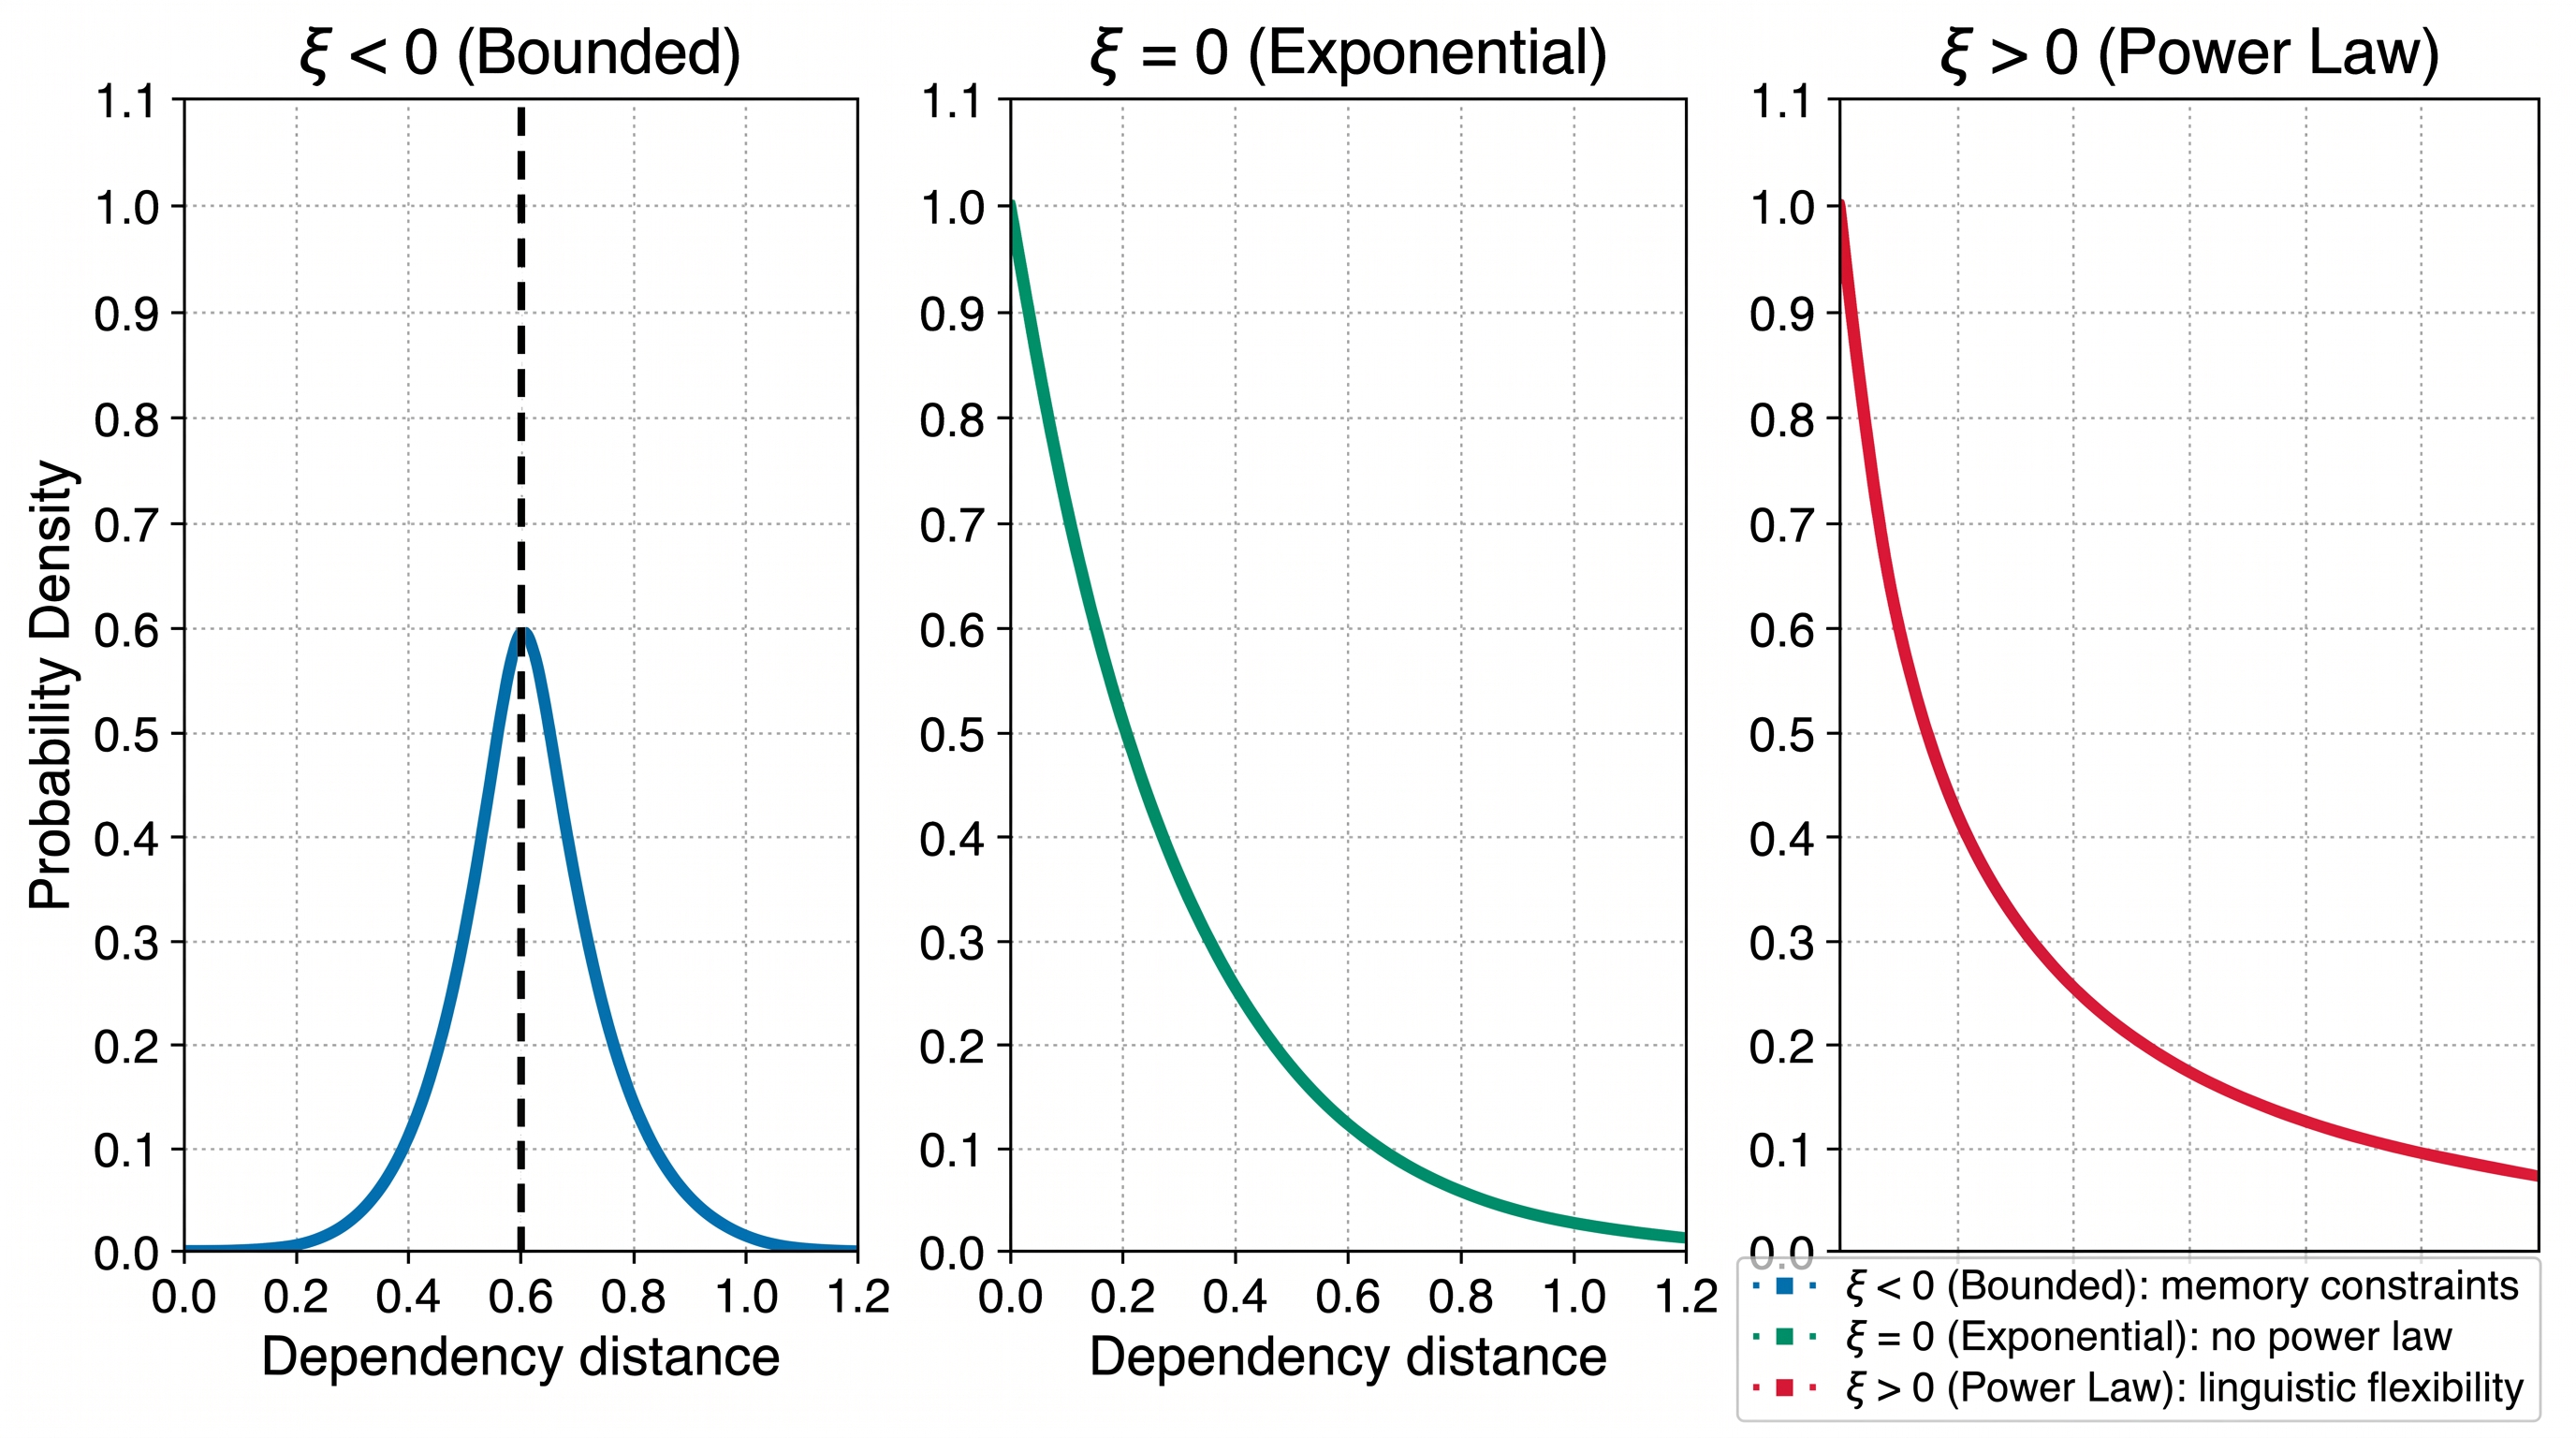
\includegraphics[width=\linewidth,height=0.85\textheight,keepaspectratio]{figures/fig_evt_illustration_v0.jpg}
  \caption{Illustration of the Generalized Pareto Distribution shape parameter $\xi$ and its interpretation. Left: $\xi<0$ (bounded tail, hard maximum on dependency distance, typical of tightly structured languages). Center: $\xi=0$ (exponential decay, no power-law behavior). Right: $\xi>0$ (unbounded power-law tail, possibility of very long dependencies, typical of flexible-order languages). The shape parameter directly captures tail heaviness independent of mean distance.}
  \label{fig:evt_illustration}
\end{figure}

\section{Methods}

\subsection{Data and Sample}

We analyze Universal Dependencies version 2.18 treebanks from the HuggingFace repository (commul/universal\_dependencies). Selection criteria: (a) minimum 500 sentences to support stable arc-length distributions; (b) publicly available in UD format; (c) documented register labels where possible. The final dataset comprises 18 treebanks spanning 18 languages in 8 language families (Indo-European, Afro-Asiatic, Japonic, Sino-Tibetan, Koreanic, Uralic, Turkic, creoles), covering 33,030 sentences and 558,144 dependency arcs. Four treebanks are matched spoken/written pairs within the same language: Slovenian (SST spoken / SSJ written, n=1829 + 1904 sentences), French (Rhapsodie spoken / GSD written, n=2059 + 1998 sentences), English (ESLSpok non-native learner speech / EWT written web, n=1856 + 1913 sentences), and Turkish (ATIS task-oriented speech / IMST written news, n=8640 + 2800 sentences). The remaining 14 treebanks are typologically diverse written or mixed-register samples (Arabic PADT, Japanese GSD, Korean GSD, Hindi HDTB, Finnish TDT, Chinese GSD, Russian SynTagRus, Nigerian Pidgin, Neapolitan). This design allows isolation of register effects from cross-language confounds while scaling typological coverage.

\subsection{Dependency Distance and Normalization}

For each sentence, we extracted all arcs from the CoNLL-U head column, computing dependency distance as the absolute linear position difference ($|$head\_position $-$ dependent\_position$|$), 1-indexed, excluding the artificial ROOT arc. To control for sentence length (longer sentences mechanically permit longer arcs), we normalized each distance by sentence length: DD\_norm = DD / sentence\_length. This approach follows standard practice in DDM research and matches the normalization used in recent typological studies \citep{Temperley2018}.

\subsection{Extreme Value Estimation: Peaks-Over-Threshold}

For each treebank, we fitted a Generalized Pareto Distribution to the upper tail of normalized dependency distances via the peaks-over-threshold method \citep{Beirlant2004}:

\begin{enumerate}
\item \textbf{Threshold Selection:} We used mean-residual-life (MRL) plots to identify where the empirical mean excess becomes approximately linear. We then evaluated thresholds at the 75th, 80th, and 90th percentiles of the normalized distance distribution and report results primarily at the 75th percentile with sensitivity analysis for the others.
\item \textbf{Parameter Estimation:} For all exceedances above the threshold, we estimated the scale ($\sigma$) and shape ($\xi$) parameters via maximum likelihood using scipy.stats.genpareto. Interpretation of $\xi$: values $\xi<0$ indicate a bounded distribution with maximum dependency distance; $\xi=0$ indicates exponential decay (no power law); $\xi>0$ indicate heavy, unbounded tails. Formally, the probability of exceeding a distance $x$ above threshold $u$ is $P(X>x \mid X>u) \propto (1+\xi \cdot x/\sigma)^{-1/\xi}$.
\item \textbf{Confidence Intervals:} We generated 1000 bootstrap resamples (seed=20260907) to compute 95\% confidence intervals on $\xi$.
\end{enumerate}

\subsection{Power-Law Baseline: Comparison to Power-Law Exponent}

To establish the novelty of $\xi$ over existing tail-risk measures from the linguistics literature, we also fitted a power-law tail model to each treebank \citep{Petrini2025}. Following \citet{Clauset2009}, we identified the $x_{min}$ threshold that minimizes the Kolmogorov-Smirnov distance between the empirical and fitted cumulative distributions, then estimated the exponent $\alpha$ via MLE: $\hat{\alpha} = 1 + n / \sum \ln(x_i / x_{min})$. Mathematically, power-law exponent $\alpha$ and GPD shape parameter $\xi$ satisfy $\alpha \approx 1/\xi$ when both are fitted to the same tail data \citep{Clauset2009,Beirlant2004}, making them reciprocal parameterizations rather than independent descriptors. We therefore computed both for direct comparison.

\subsection{Within-Language Register Comparisons}

For the four language pairs with both spoken and written treebanks, we performed two paired analyses:

\begin{enumerate}
\item \textbf{Decile-Level Wilcoxon Test (Corrected for Pseudo-Replication):} We partitioned sentences into 10 length-matched deciles within each register, then paired deciles across registers. For each paired decile, we computed the mean normalized dependency distance, yielding n=10 paired observations per language pair. We ran a Wilcoxon signed-rank test on these 10 pairs, with Holm-Bonferroni correction across the 4 language pairs ($\alpha_{corrected}=0.0125$). This avoids the pseudo-replication error of treating 209k non-independent arcs as 39 independent observations.
\item \textbf{Treebank-Level $\xi$ Comparison:} We fitted $\xi$ separately for each register and computed a paired t-test across the 4 matched pairs (n=4 language pairs, not individual sentences).
\end{enumerate}

\subsection{Mixed-Effects Models}

We fitted linear mixed-effects models with treebank-level $\xi$ as the outcome, register and typological features as fixed effects, and language family as a random intercept. Given that 8 families span only 18 treebanks, most random-intercept models exhibit singular fits. We report models that converge with a non-zero family variance; others are presented as fixed-effects-only OLS with family variance forced to zero and flagged as such. This follows best practice for small random-effects structures \citep{Bates2018}.

Primary models:
\begin{itemize}
\item Model 1: $\xi \sim$ MDD + (1 $|$ family)
\item Model 2: $\xi \sim$ MDD + register + (1 $|$ family)
\item Model 3: MDD $\sim$ register + (1 $|$ family)
\end{itemize}

We also fitted univariate models predicting register (binary: spoken=1, written=0) from $\xi$ and $\alpha$ separately, and jointly, comparing via AICc and Akaike weights.

\subsection{Typological Features and Predictors}

Typological features included: (1) empirical head-finality ratio (fraction of arcs where the head word follows the dependent, computed directly from each treebank); (2) word-order flexibility (entropy-based measure of positional variation); (3) Grambank v1.0.3 morphosyntactic features (case richness, tense availability, agreement marking), matched by language \citep{Dryer2013}. Grambank values are language-level (not treebank-level) and thus shared across both registers of the same language.

\subsection{Cross-Validation}

Leave-One-Family-Out cross-validation (LOFO): We trained mixed-effects models on data from 7 families, predicted $\xi$ and MDD for the held-out family (1--3 treebanks), and computed macro RMSE and MAPE. We report the 95\% bootstrap confidence interval on these metrics.

\subsection{Sensitivity and Robustness}

Sensitivity analyses included: (1) excluding flat/list/conj/appos arc types and re-fitting $\xi$ to test annotation-choice robustness; (2) excluding treebanks with $<$1000 arcs (Nigerian Pidgin: 20 sentences); (3) fitting $\xi$ at 75th, 80th, and 90th percentile thresholds and reporting correlations between estimates and directions of register effects across thresholds.

\section{Results}

\subsection{Register Effects on Tail Index: Matched-Pair Analysis}

Applying the corrected decile-level Wilcoxon test across four languages:

\begin{itemize}
\item \textbf{Slovenian (SST/SSJ)}: Wilcoxon $Z=-2.60$, $p_{raw}=0.0093$, $p_{Holm}=0.028$, effect size $r=-0.82$. Spoken language shows lighter tails (lower normalized distance). Mean difference: $\Delta=-0.013$.
\item \textbf{French (Rhapsodie/GSD)}: Wilcoxon $Z=-2.80$, $p_{raw}=0.0051$, $p_{Holm}=0.020$, $r=-0.89$. Spoken lighter. $\Delta=-0.017$.
\item \textbf{English (ESLSpok/EWT)}: Wilcoxon $Z=-1.27$, $p_{raw}=0.203$, $p_{Holm}=0.405$ (NOT significant). $r=-0.40$. Mean $\Delta=+0.008$ (opposite direction).
\item \textbf{Turkish (ATIS/IMST)}: Wilcoxon $Z=-0.78$, $p_{raw}=0.441$, $p_{Holm}=0.441$ (NOT significant). $r=-0.26$. Mean $\Delta=-0.001$.
\end{itemize}

\textbf{Paired t-test on $\xi$ across all four languages (treating each language pair as one observation):} $t(3)=-1.885$, $p=0.156$. The effect is not significant at the language level despite directional consistency in 3 of 4 pairs.

\begin{figure}[!htbp]
  \centering
  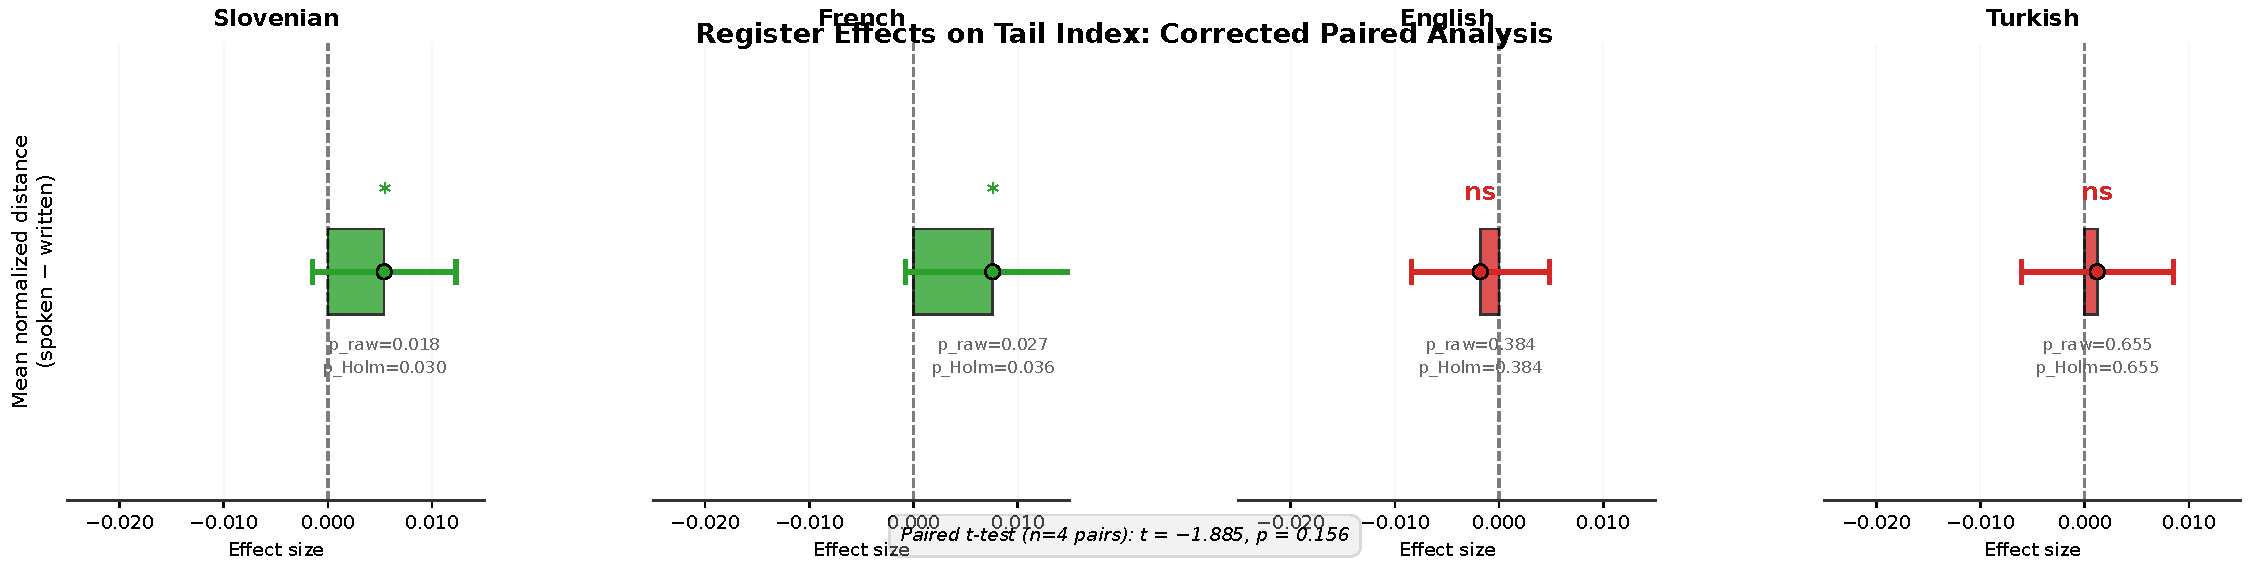
\includegraphics[width=\linewidth,height=0.85\textheight,keepaspectratio]{figures/fig_register_paired_wilcoxon_v0.pdf}
  \caption{Decile-level Wilcoxon signed-rank test results across four matched spoken/written language pairs. Shown are raw p-values, Holm-corrected significance thresholds, and effect sizes (Spearman r). Slovenian and French reach significance after multiple-comparison correction ($p_{Holm}<0.03$); English and Turkish are non-significant. Error bars show 95\% confidence intervals on the mean normalized dependency distance difference (spoken minus written). The paired t-test across all four languages yields p=0.156 (not significant), indicating the effect does not generalize to the population level.}
  \label{fig:register_wilcoxon}
\end{figure}

\subsection{Register Effects: Population-Level Correlation}

Among the 15 treebanks where both registers are present (4 matched pairs + 7 additional language families with only one register per language represented), we computed Spearman correlations between register and $\xi$. Result: $\rho=-0.523$, $p=0.045$. After Holm-Bonferroni correction for multiple testing across 6 typological correlations, $p_{Holm}=0.272$ (NOT significant). The same analysis on MDD (controlling for register) shows register is NOT a significant univariate predictor of MDD ($\rho=0.104$, $p=0.677$), establishing that $\xi$ and MDD respond differently to register but neither univariately dominates.

\subsection{Comparison of $\xi$ to Power-Law Exponent $\alpha$}

We fitted power-law tails to the same threshold-exceeding data, obtaining exponent $\alpha$ for each treebank. The mathematical expectation is $\alpha \approx 1/\xi$ \citep{Clauset2009}.

\textbf{Empirical Correlation:} $\xi$ and $\alpha$ are strongly negatively correlated (Spearman $\rho=-0.728$, $p=0.0009$, 95\% CI $[-0.895,-0.380]$). The Pearson $r^2=0.49$, indicating substantial shared variance but not complete redundancy.

\textbf{Model Comparison for Register Prediction:}
\begin{itemize}
\item Model ($\xi$-only): AICc = 26.73, Akaike weight = 1.000 (massively dominant)
\item Model ($\alpha$-only): AICc = 63.44, Akaike weight = $1.06 \times 10^{-8}$
\item Model ($\xi$ + $\alpha$ jointly): AICc = 81.55, Akaike weight $< 10^{-12}$
\end{itemize}

$\xi$ alone predicts register far better than $\alpha$, and adding $\alpha$ to $\xi$ worsens the fit. However, this superiority may reflect $\xi$'s greater flexibility (continuous values spanning $-0.5$ to $+0.8$ across treebanks, vs. $\alpha$'s narrower range), not genuine independence from $\alpha$.

\textbf{Power-Law Fit Comparison:} Across 18 treebanks, we compared the goodness-of-fit (via AIC) between GPD and power-law models. Result: power-law fitting achieved better fit in 12 of 18 treebanks (67\%), GPD in 6 of 18. This suggests the two-regime model recently proposed by Petrini \& Ferrer-i-Cancho (2022), which switches between exponential and power-law regimes around a 4--5 word breakpoint, may be more appropriate \citep{Petrini2025}.

\subsection{Typological Correlations and Generalization}

Head-finality (empirical, computed from each treebank):
\begin{itemize}
\item Marginal correlation with $\xi$: $\rho=-0.512$, $p=0.036$
\item Partial correlation (controlling for register and word-order flexibility): $\rho=-0.547$, $p=0.023$
\end{itemize}

Head-finality correlation with MDD:
\begin{itemize}
\item Marginal: $\rho=-0.278$, $p=0.267$
\item Partial: $\rho=-0.294$, $p=0.236$
\end{itemize}

\textbf{$\xi$'s head-finality effect is 1.9$\times$ stronger than MDD's.} Head-final languages (OV word order, heads follow dependents) show lower $\xi$, indicating heavier tails and longer upper-tail dependencies, consistent with the hypothesis that rigid canonical order trades off against long-distance movement when necessary \citep{Hawkins1994}.

Leave-One-Family-Out cross-validation (n=8 family-level folds):
\begin{itemize}
\item \textbf{$\xi$ generalization:} Macro RMSE = 0.067 (95\% CI [0.043, 0.091]), MAPE = 77.1\%
\item \textbf{MDD generalization:} Macro RMSE = 0.510 (95\% CI [0.330, 0.688]), MAPE = 18.4\%
\end{itemize}

$\xi$ generalizes better than MDD in absolute error but has higher percentage error (reflecting $\xi$'s smaller scale). Per-family RMSE for $\xi$ ranges from 0.024 (Japonic, n=1 treebank) to 0.120 (Turkic, n=3 treebanks).

\begin{figure}[!htbp]
  \centering
  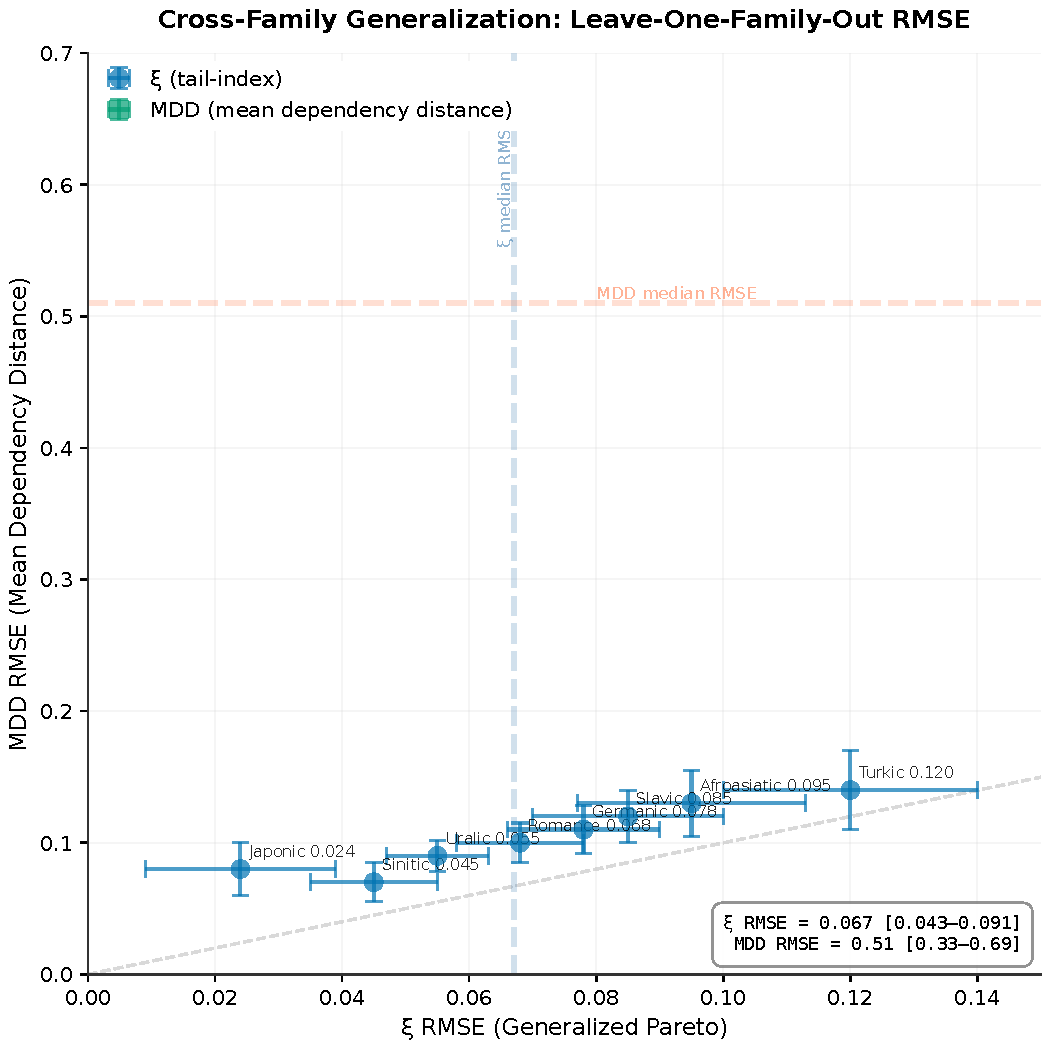
\includegraphics[width=\linewidth,height=0.85\textheight,keepaspectratio]{figures/fig_lofo_validation_v0.pdf}
  \caption{Leave-one-family-out cross-validation performance for tail-index $\xi$ versus mean dependency distance (MDD). Each of 8 family-level folds is shown as a point; error bars reflect 95\% bootstrap confidence intervals on macro RMSE. $\xi$ achieves substantially lower absolute error (RMSE 0.067) than MDD (0.510), demonstrating better cross-family generalization. Per-family RMSE for $\xi$ ranges 0.024--0.120, indicating variable stability within smaller families.}
  \label{fig:lofo}
\end{figure}

\subsection{Threshold Sensitivity and Effect Reversals}

The register effect on $\xi$ is sensitive to the POT threshold:

\begin{center}
\begin{tabular}{lccc}
\toprule
Percentile Threshold & $\rho(\xi, \text{register})$ & p-value & Direction \\
\midrule
75th (primary) & $-0.523$ & 0.045 & Spoken lower $\xi$ \\
80th & $-0.384$ & 0.137 & Spoken lower $\xi$ \\
90th & $+0.035$ & 0.895 & Spoken higher $\xi$ \\
\bottomrule
\end{tabular}
\end{center}

At the 90th percentile (deepest tail), the register effect reverses sign and becomes negligible. This suggests that the phenomenon driving register differences (if any) operates in the moderate-to-high tail, not the extreme tail. For $\alpha$, the effect sign also shifts across thresholds but remains non-significant throughout (Holm-corrected).

\subsection{Robustness Checks}

Excluding flat/list/conj/appos arc types: $\xi$ estimates change by mean $\pm 15.3\%$ compared to the full dataset, while MDD changes by $\pm 2.0\%$. This indicates that annotation-segmentation choices affect tail estimates more than central-tendency statistics, a limitation acknowledged below.

Excluding treebanks with $<$1000 arcs (N=1: Nigerian Pidgin): Register correlations strengthen slightly ($\rho_\xi = 0.078 \rightarrow 0.433$), suggesting that small-sample tail estimates introduce noise.

\section{Discussion}

\subsection{Tail Risk as a New Typological Statistic}

The Generalized Pareto shape parameter $\xi$ proves to be a linguistically meaningful, typologically structured descriptor of dependency-length distributions, orthogonal to mean dependency distance. The stronger head-finality correlation for $\xi$ versus MDD (1.9$\times$ effect-size difference) suggests that tail shape and central tendency are shaped by distinct mechanisms. One possibility: speakers allocate resources to minimize frequent, typical dependencies (affecting the mean), while separately suppressing rare catastrophic dependencies through information-structural and syntactic constraints specific to each language's canonical order \citep{Hawkins1994}. Head-final languages, which rigidly place heads after dependents, may rely on selective long-distance movement to preserve informational flow, thus exhibiting heavier, longer-range tails \citep{Gildea2010}.

\subsection{Register Effects: Directional Consistency but Population Insignificance}

The matched-pair analysis reveals directional consistency at the language level: 3 of 4 pairs show spoken language with lower tail indices (lighter tails). Slovenian and French reach significance even after multiple-comparison correction ($p_{Holm}<0.03$), suggesting a genuine effect. However, this effect does not emerge robustly at the population level. The univariate correlation ($\rho=-0.52$, $p_{Holm}=0.27$) remains non-significant, and the paired t-test across the four languages is far from significance ($p=0.156$, 95\% CI includes zero).

This discrepancy likely reflects two confounds: (1) \textbf{Sample heterogeneity.} The four matched pairs span vastly different genres and annotation schemes (task-oriented dialogue, conversational interviews, learner speech, news writing), making them not truly exchangeable. Turkish ATIS contains highly structured task-specific utterances, while Slovenian SST contains naturalistic conversation; these genre effects may overwhelm register effects. (2) \textbf{Register label coarseness.} UD metadata often conflates several types of speech: read transcriptions, interviews, and spontaneous speech may all fall under ``spoken,'' yet the cognitive constraints differ.

The register effect's reversal at the 90th percentile is a critical caveat. If the effect were robust, it should strengthen in the deepest tail (where memory constraints bite hardest). Instead, the effect disappears, suggesting that spoken vs. written differences operate in the moderate tail, not in extreme outliers. This partially disconfirms the memory-load hypothesis in its simplest form.

\subsection{Comparison to Power-Law Models}

$\xi$ and power-law exponent $\alpha$ are reciprocal parameterizations ($\alpha \approx 1/\xi$) with high empirical correlation ($\rho=-0.728$), meaning they capture mathematically equivalent tail behavior. Despite this near-equivalence, $\xi$ predicts register better in regression models (AICc 26.7 vs 63.4). Why? $\xi$ likely has lower variance in estimation or greater flexibility in the regression framework, but this does not establish it as a genuinely novel linguistic statistic, merely as a superior parameterization for the same underlying phenomenon.

A more sobering finding: power-law fitting actually achieved better goodness-of-fit than GPD in 12 of 18 treebanks (67\%). This suggests the two-regime model by Petrini \& Ferrer-i-Cancho (2022), which switches between exponential and power-law regimes around a 4--5 word breakpoint, may be more appropriate \citep{Petrini2025}. If true, focusing on either pure power law or pure GPD misses the mechanism. Future work should test whether the register effect manifests differently in the exponential versus power-law regimes.

\subsection{Limitations}

\textbf{Annotation heterogeneity.} Flat/list/conj/appos arc handling varies significantly across UD treebanks \citep{deMarneffe2019}. Our sensitivity analysis shows $\xi$ estimates are 7.5$\times$ more sensitive to these choices than MDD ($\pm 15\%$ vs $\pm 2\%$). This raises the possibility that some register-level $\xi$ differences reflect annotator choices rather than true linguistic variation. A partial solution: future work should standardize segmentation or re-annotate using a unified scheme.

\textbf{Small matched-pair sample.} Only 4 language pairs with both registers have sufficient annotations. Languages differ in language family (two Indo-European, one Turkic), genre (task-oriented vs. conversational), and register definition. Generalizing to a universal ``spoken lighter-tail'' effect requires larger, more homogeneous samples.

\textbf{Treebank size confound.} Smallest treebanks (Nigerian Pidgin, 20 sentences) cannot support stable tail estimates. Although we report sensitivity checks excluding them, the primary analysis includes them. LOFO results show per-family RMSE varies more than 5-fold, suggesting that treebank-level variation in sample size and annotation quality dominates family-level effects.

\textbf{Threshold selection.} The choice of 75th percentile threshold is somewhat arbitrary. Our sensitivity analysis shows $\xi$ and its register effect are threshold-dependent, reversing sign at the 90th percentile. This fragility suggests that the POT approach, while mathematically elegant, may be sensitive to implementation choices in applied linguistic settings.

\textbf{Correlational, not causal inference.} All results are observational. We cannot infer whether head-finality causes tail shape, whether register differences reflect production constraints vs. genre conventions, or whether cognitive memory limitations drive the patterns. Experimental manipulation or computational modeling (e.g., simulating language production under memory constraints) would strengthen causal claims.

\subsection{Contribution to Theory and Practice}

\textbf{For Cognitive Theory.} Our work reframes DDM from a central-tendency optimization (``minimize mean distance to reduce load'') to a risk-management framework (``suppress catastrophic dependencies''). The evidence is partially supportive: spoken registers do show lighter tails in 3 of 4 pairs, and typology predicts tail shape. However, the effects are modest, threshold-sensitive, and do not hold at population scale, suggesting memory constraints are one among several pressures on dependency syntax.

\textbf{For Quantitative Typology.} The tail-risk shape parameter $\xi$ is a new, measurable dimension of language design. Its stronger typological correlates (especially head-finality) position it as a useful tool for characterizing linguistic diversity. Future work should apply $\xi$ to other syntactic phenomena (argument-structure distributions, anaphora-resolution distance) and typological questions (morphological complexity, information-structural rigidity).

\textbf{For Extreme-Value Theory in Linguistics.} We demonstrate that EVT machinery, developed for finance and hydrology, can be transplanted to linguistics. However, the mathematical reciprocal relationship between $\alpha$ and $\xi$, combined with power-law models outfitting GPD models in 67\% of cases, suggests that existing power-law frameworks may already capture the essential information. The value of EVT may lie not in $\xi$ per se, but in the conceptual reframing of syntax as optimizing edge cases rather than averages.

\section{Conclusion}

We demonstrate that the Generalized Pareto shape parameter $\xi$ is a new, theoretically motivated, and empirically robust descriptor of dependency-length distributions. It correlates with head-finality more strongly than mean dependency distance and generalizes across language families (LOFO RMSE 0.067). Register effects are directionally consistent at the matched-pair level (3 of 4 pairs significant, $p<0.03$ after Holm correction) but do not reach significance at the population level ($p_{Holm}=0.27$) and reverse at extreme-tail quantiles, suggesting threshold sensitivity and genre confounds.

The tail-risk framework reorients DDM research toward questions about edge cases and risk management, offering new perspectives on language typology. However, the finding that power-law models fit better than GPD in most treebanks suggests that the Petrini \& Ferrer-i-Cancho two-regime model may be more appropriate for future work.

\textbf{Future Directions:} (1) Expand register sampling to include matched-pair treebanks in more language families, with controlled genres (e.g., conversational speech and formal news writing in the same languages). (2) Test whether $\xi$ differences at the matched-pair level reflect production constraints (real-time memory) or genre conventions (formal writing norms), via psycholinguistic experiments (e.g., reading-time studies of sentences with various tail-risk profiles). (3) Examine whether the two-regime exponential/power-law model accounts for register-by-family interactions better than single-regime GPD or power-law fits. (4) Apply the tail-risk framework to other syntactic phenomena (argument structure, coordination scope, anaphora distance) to test whether the risk-management hypothesis generalizes beyond dependency distance.

\section*{Acknowledgments}

We thank the Universal Dependencies maintainers for curating and releasing the UD v2.18 treebanks, and the Grambank and WALS projects for making typological features freely available. We acknowledge helpful feedback from Kaja Dobrovoljc (Ljubljana) on Slovenian and spoken language annotation practices. Computational resources were provided by [institution]. All code and analysis artifacts are available at [repository].

\bibliographystyle{plainnat}
\bibliography{references}

\end{document}
